\documentclass{loyola-beamer}
\renewcommand{\titlelogo}{logo/luc-rev.svg}
\renewcommand{\slidelogo}{logo/luc.svg}
\usepackage{physics}
\usepackage{graphicx}
\usepackage{hyperref}

\renewcommand{\slidefoot}{Department of Physics -- PHYS422}
\def\c#1{\texttt{#1}}

\title{How The Atomic Bombs Were Made ?}
\subtitle{A deep dive into the physics behind disaster of atomic bombs}
\author{Ammar S. Alfaifi}
\date{\today}
\institute{KFUPM}

\begin{document}

\begin{titleframe}{}
	\maketitle
\end{titleframe}

\begin{frame}{Contents}
	\tableofcontents
\end{frame}

% Start of the main contents
\begin{frame}{Introduction}
\end{frame}

\begin{frame}
	\begin{itemize}
		\item In 1942, before the Manhattan Project, Robert Oppenheimer held conferences where physicists discussed nuclear bomb design issues.
		\item A gun-type design was initially chosen, where two sub-critical masses of plutonium would be brought together by firing a "bullet" into a "target".
		\item The alternative implosion-type design, suggested by Richard Tolman, was considered far more complex and received scant consideration.
	\end{itemize}
\end{frame}

\section{Thin Man}

\begin{frame}
	\begin{itemize}
		\item In early 1943, Oppenheimer prioritized the gun-type weapon but created the E-5 Group at Los Alamos to investigate implosion as a hedge against predetonation.
		\item Implosion-type bombs were determined to be more efficient in terms of explosive yield per unit mass of fissile material due to compressed fissile materials reacting more rapidly and completely.
		\item However, the plutonium gun-type bomb received the bulk of the research effort due to less uncertainty involved, with the assumption that the uranium gun-type bomb could be easily adapted from it.
	\end{itemize}
\end{frame}

\begin{frame}
	\begin{figure}
		\begin{center}
			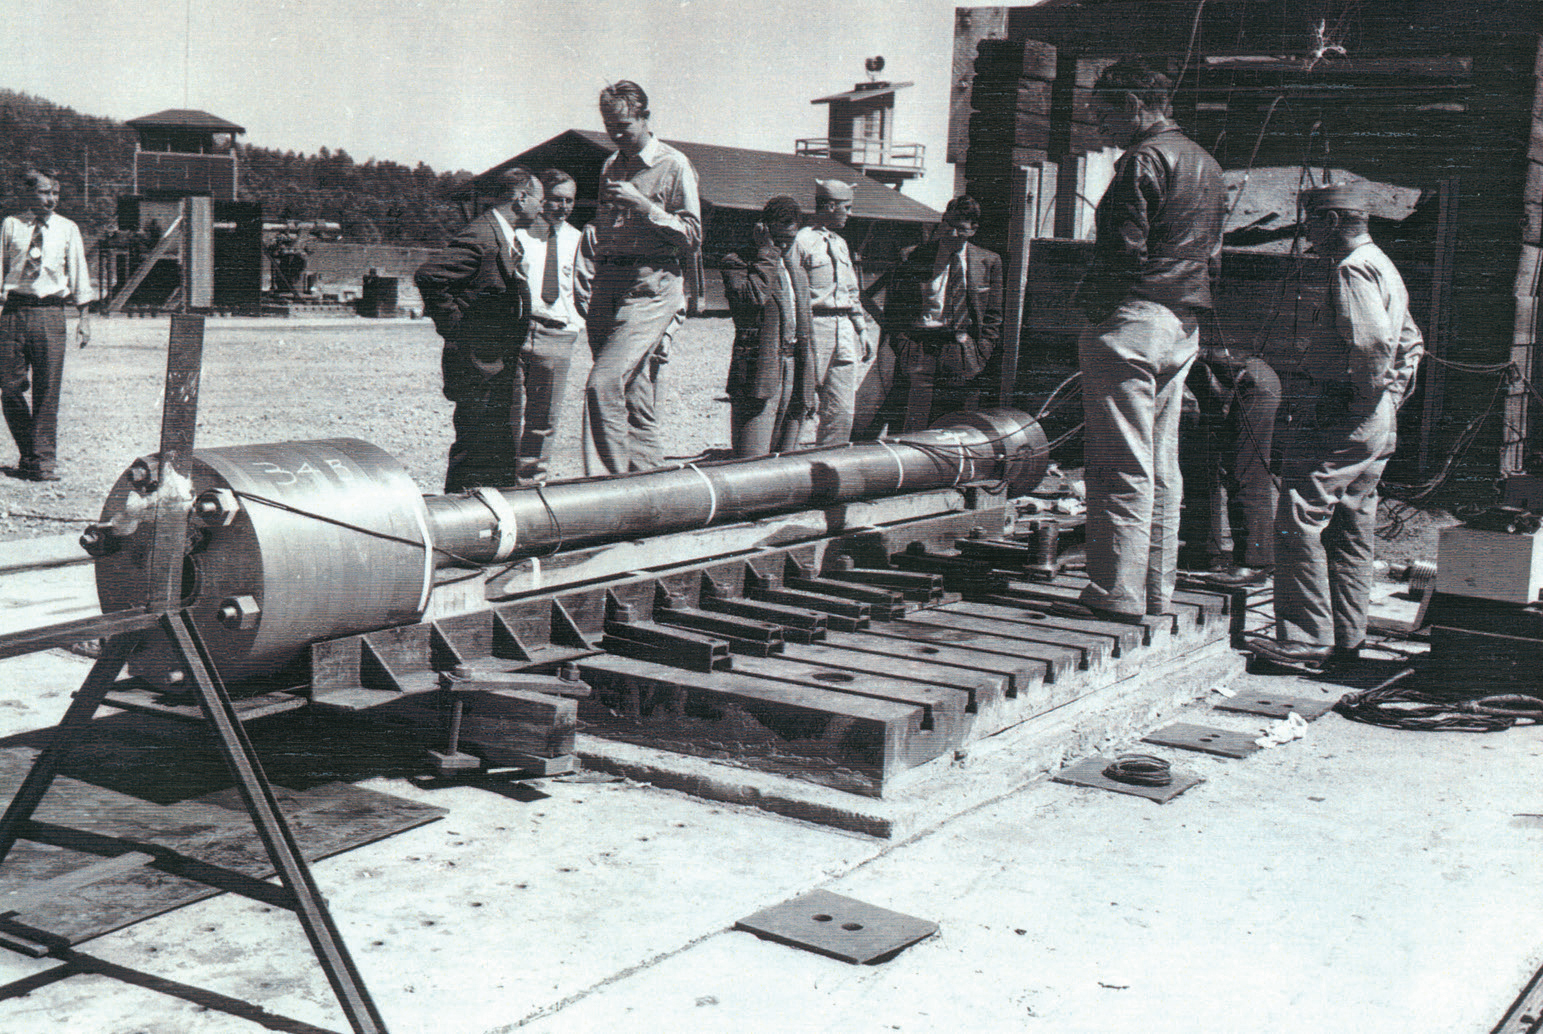
\includegraphics[width=0.7\textwidth]{./figures/Thin_Man_testing_at_Anchor_Ranch.jpg}
		\end{center}
		\caption{A prototype of the "Thin Man" gun being tested at Anchor Ranch, at Los Alamos.}\label{fig:thin man img}
	\end{figure}
\end{frame}

\begin{frame}
	\begin{itemize}
		\item "Thin Man" was an early nuclear weapon design proposed before plutonium breeding.
		\item It assumed plutonium could be assembled by a gun-type method, requiring a "bullet" speed of at least 910 m/s.
		\item Dimensions: 5.2 m long, 0.97 m wide tail and nose, 0.58 m midsection.
		\item Weight: approximately 3,600 kg.
		\item No USAAF aircraft could carry it without modifications.
		\item Avro Lancaster (10 m bomb bay) or modified Boeing B-29 Superfortress were suggested.
		\item B-29 modification involved removing part of the bulkhead and oxygen tanks (Serial No. 42-6259).
	\end{itemize}
\end{frame}

\begin{frame}
	\begin{figure}
		\begin{center}
			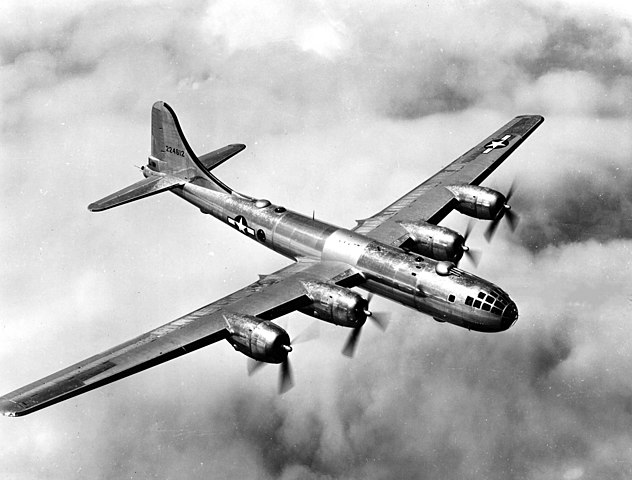
\includegraphics[width=0.6\textwidth]{figures/632px-B-29_in_flight.jpg}
		\end{center}
		\caption{A USAAF B-29 Superfortress. B-29s dropped the atomic bombs on Hiroshima and Nagasaki, the only aircraft ever to drop nuclear weapons in combat.}
	\end{figure}
\end{frame}

\subsection{Issues}

\begin{frame}{Predetonation}
	\begin{itemize}
		\item Experiments in April 1944 by Emilio G. Segrè's group at Los Alamos showed reactor-produced plutonium contained the isotope plutonium-240.
		\item Plutonium-240 has a high spontaneous fission rate, increasing the risk of predetonation.
		\item This meant the plutonium would likely predetonate and blow itself apart during critical mass formation.
		\item The distance required to avoid predetonation would need an impractically long gun barrel for any bomber.
	\end{itemize}
\end{frame}

\begin{frame}
	\begin{itemize}
		\item The only viable option was the more difficult implosion method.\cite{Hoddeson1993}
		\item At a meeting on July 17, 1944, it was agreed that gun-type work would focus on the \texttt{Little Boy} uranium design.
		\item Almost all Los Alamos research was re-oriented toward solving the implosion problems for the \texttt{Fat Man} plutonium bomb.
	\end{itemize}
\end{frame}

\begin{frame}
	\begin{figure}
		\includesvg[width=0.45\textwidth]{figures/Nuclear_predetonation.svg}
		\caption{If two pieces of subcritical material are not brought together fast enough, nuclear predetonation can occur, whereby a smaller explosion than expected will blow the bulk of the material apart.}
	\end{figure}
\end{frame}

\begin{frame}
	\begin{equation*}
		{ }_{92}^{238} \mathrm{U}+{ }_0^1 \mathrm{n} \longrightarrow{ }_{92}^{239} \mathrm{U} \xrightarrow[23.5 \text { min }]{\beta^{-}}{ }_{93}^{239} \mathrm{~Np} \xrightarrow[2.3565 \mathrm{~d}]{\beta^{-}}{ }_{94}^{239} \mathrm{Pu}
	\end{equation*}
	\vfill
	Neutrons from the fission of uranium-235 are captured by uranium-238 nuclei to form uranium-239; a beta decay converts a neutron into a proton to form neptunium-239 (half-life 2.36 days) and another beta decay forms plutonium-239.\cite{Greenwood1997}
\end{frame}

\begin{frame}
	\begin{tabular}{|l|l|l|l|}
		\hline
		Isotope                 & Decay mode                      & Half-life (years) & Spontaneous fission $n$ (1/(g·s)) \\
		\hline
		\textsuperscript{238}Pu & alpha to \textsuperscript{234}U & 87.74             & 2600                              \\
		\hline
		\textsuperscript{239}Pu & alpha to \textsuperscript{235}U & 24100             & 0.022                             \\
		\hline
		\textsuperscript{240}Pu & alpha to \textsuperscript{236}U & 6560              & 910                               \\
		\hline
	\end{tabular}
\end{frame}

\section{References \& Conclusion}

% --- Conclusion --- %
\begin{frame}{Conclusion}
	\begin{itemize}
		\item Majorana fermion braiding explored through a series of measurements.
		\item Ancilla Majorana fermions contribute to robustness.
		\item Error assessment provides insights into the fidelity of braiding.
	\end{itemize}
\end{frame}

% --- References --- %
\begin{frame}{References}
	\bibliographystyle{plain}
	\bibliography{references}
\end{frame}

% ---- The End ---- %
\begin{titleframe}{Thank you for listening.}
\end{titleframe}

\end{document}
